% 2010 年安徽卷文科第 17 题：椭圆 E、焦点 F1、F2 与 ∠F1AF2 的角平分线。
% 来源 PDF：普通高考/2010/2010安徽文.pdf，SHA-256 1bd928e09356787e648fa9efb9b4c1525f26334f65b08ba82fc736ebb110a4cb。
% 原页：第 1 页（A3 三栏）第 3 栏中部，书页码 571。
% 重绘依据：椭圆 x²/16+y²/12=1，A(2,3)，F1(−2,0)，F2(2,0)；
%   角平分线方向为 (−1,−2)，过 A 后与椭圆另一交点为 (−22/19,−63/19)，按计算结果绘制。
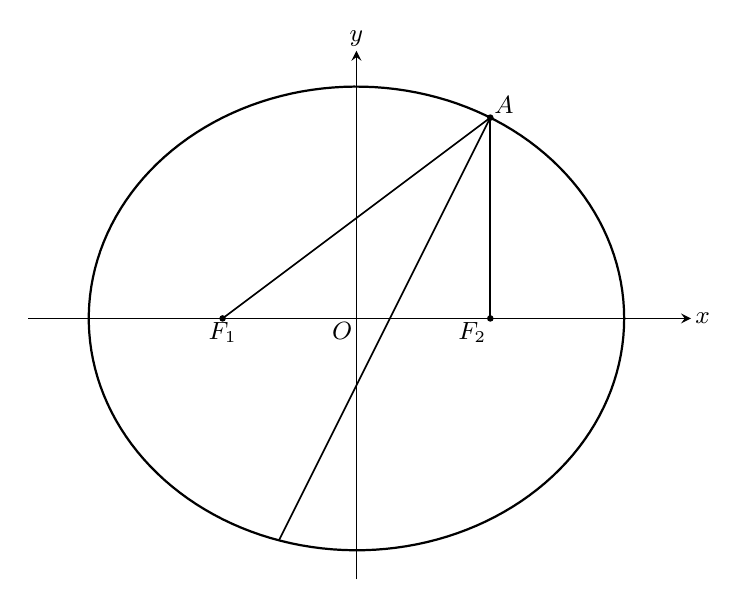
\begin{tikzpicture}[semithick, scale=0.85, every node/.style={inner sep=1.2pt, font=\small}]
  \draw[-stealth] (-4.9,0) -- (5.0,0) node[right] {$x$};
  \draw[-stealth] (0,-3.9) -- (0,4.0) node[above] {$y$};
  \draw[thick,domain=0:360,samples=160] plot ({4*cos(\x)},{3.4641*sin(\x)});
  \coordinate (A) at (2,3);
  \coordinate (F1) at (-2,0);
  \coordinate (F2) at (2,0);
  \coordinate (P) at (-1.1579,-3.3158);
  \draw (A) -- (F1);
  \draw (A) -- (F2);
  \draw (A) -- (P);
  \fill (A) circle (1.4pt);
  \fill (F1) circle (1.4pt);
  \fill (F2) circle (1.4pt);
  \node[above right] at (A) {$A$};
  \node[below] at (F1) {$F_1$};
  \node[below left] at (F2) {$F_2$};
  \node[below left] at (0,0) {$O$};
\end{tikzpicture}
